% !TeX root = main.tex
\chapter{随机变量与分布函数}
\section{随机变量及其分布}
随机变量是一个事件到实数(轴上的Borel集)的映射,目的在于数值化样本点。之所以掷骰子点数的期望看起来不自然,
就是因为他依赖于随机变量对事件的映射。

随机变量还允许我们对变量进行数学运算。\[
    \xi \sim N(0,1) \iff \xi+1 \sim N(1,1)
\]

分布是随机变量的概率性质。

分布函数是随机变量取值小于等于某个特定值的概率。在离散型随机变量里,分布列是随机变量取特定值的结果。在连续型随机变量里,
概率密度函数是分布函数的导数。二者都把概率刻画成一定的直观测度,但截然不同。不可能通过趋于无穷的分布列逼近概率密度函数,
因为此时分布列必然所有元素都趋于0。但分布函数是可以由离散向连续逼近的。

% TODO: 密度函数的基本性质和分布函数的基本性质与判定,权当参考
% TODO: 增加二项分布逼近超几何分布
以下介绍离散与连续相对应的总共六种分布:

\subsection{离散型随机变量}
% 伯努利试验
% 二项分布、超几何分布的简单介绍(严谨化 P181 25)
\subsubsection{几何分布}

\begin{definition}{几何分布}
    在成功的概率为\(p\) 的伯努利试验中,若以第\(\zeta\)
    记第一次成功出现时的试验次数为随机变量\(\zeta\),则\(\zeta\) 服从几何分布:
    \[
        \P{\zeta=k} = (1-p)^{k-1} p, \quad k=1,2,\ldots
    \]
\end{definition}

% 几何分布的无记忆性

\subsubsection{帕斯卡分布}

\begin{definition}{帕斯卡分布}
    在成功的概率为\(p\) 的伯努利试验中,若以第\(\zeta\) 记第\(r\)
    次成功出现时的试验次数为随机变量\(\zeta\),则\(\zeta\) 服从帕斯卡分布:
    \[
        \P{\zeta=k} = \binom{k-1}{r-1} p^r
        (1-p)^{k-r}, \quad k=r,r+1,\ldots
    \]
\end{definition}

% TODO:负二项分布?有什么用?

帕斯卡分布与几何分布有以下关系:若以\(\nu_{i}\) 记第\(i-1\) 次成功后第一次试验算起至第\(i\)
次成功为止进行的的试验次数,则\(\nu_{i}\) 相互独立、服从几何分布,且:
\[
    \zeta = \nu_{1} + \nu_{2} + \cdots + \nu_{r}
\]

我们实际上可以从此直接推导出帕斯卡分布的概率分布:
由\(\zeta = \nu_{1} + \nu_{2} + \cdots + \nu_{r}\) 有:
\begin{align*}
    \P{\zeta=k} &=
    \sum_{\substack{i_{1}+i_{2}+\dots +i_{r}=k
    \\ i_{1},i_{2},\ldots,i_{r}\geq 1}} \P{\nu_{1}=i_{1},
    \nu_{2}=i_{2}, \ldots, \nu_{r}=i_{r}} \\
    &=\sum_{\substack{i_{1}+i_{2}+\dots +i_{r}=k
    \\ i_{1},i_{2},\ldots,i_{r}\geq 1}} P\left\{
    \nu_{1}=i_{1}\right\} \P{ \nu_{2}=i_{2} }
    \cdots \P{ \nu_{r}=i_{r} } \\
    &= \sum_{\substack{i_{1}+i_{2}+\dots +i_{r}=k
    \\ i_{1},i_{2},\ldots,i_{r}\geq 1}} p(1-p)^{i_{1}-1}
    \cdot p(1-p)^{i_{2}-1} \cdots p(1-p)^{i_{r}-1} \\
    &= \sum_{\substack{i_{1}+i_{2}+\dots +i_{r}=k
    \\ i_{1},i_{2},\ldots,i_{r}\geq 1}} p^{r} (1-p)^{k-r} \\
    &= \binom{k-1}{r-1} p^{r} (1-p)^{k-r}
\end{align*}

概率论就是这样,事情很容易变得(看起来)过分复杂\UseVerb{sad}。

\subsection{连续型随机变量}
% 伯努利试验推导泊松分布(直观+公式)
% 指数分布的直观推导与无记忆性 指数分布最小值也是指数分布
% Erlang分布的推导和指数分布的推导过来
% Erlang分布严谨化对比 习题8
% TODO: 正态分布切片还是正态分布?
% TODO: P130计算机字长造成的误差是什么分布?不是对数分布?
% TODO: P137当时间紧迫我们应该求稳还是冒险
考虑在一小时内把时间划分为\(n\) 份进行伯努利试验,并期望得到\(\lambda\)次试验结果。那么随着\(n
\to \infty\),得到结果次数\(k\) 服从的二项分布将逐渐逼近泊松分布。这就是泊松分布的意义。

\subsubsection{Erlang分布} Erlang分布是帕斯卡分布的连续型版本。
\begin{definition}{Erlang分布}
    若\(\xi(t)\) 是参数为\(\lambda t\) 的泊松过程,以\(W_{t}\) 记第\(r\) 个跳跃发生的时刻。
    则随机变量\(W_{t}\) 服从Erlang分布,其概率密度函数为:
    \[
        p(t) = \frac{\lambda^{r}}{(r-1)!} \lambda t^{r-1}
        \e^{-\lambda t},
        \quad t>0
    \]
\end{definition}

Erlang分布和指数分布的关系与几何分布和帕斯卡分布的关系类似,记\(\tau_{r}\) 是泊松过程第\(r\)
个跳跃的发生间隔,则\(\tau_{r}\) 相互独立且满足指数分布,且:
\[
    W_{t} = \tau_{1} + \tau_{2} + \cdots + \tau_{r}
\]

同样的,我们可以从此式推导出Erlang分布的概率分布:
\begin{align*}
    \P{W_{r}<t} &= \P{\tau_{1}+\tau_{2}+\cdots+\tau_{r}<t} \\
    &= \idotsint\limits_{\substack{x_{1}+x_{2}+\dots +x_{r}<t
    \\ x_{i}>0, i=1,2,\ldots,r}} p(x_{1}) p(x_{2}) \cdots p(x_{r})
    \d{x}_{1} \d{x}_{2} \cdots \d{x}_{r} \\
    &=\int_{0}^{t} \lambda \e^{-\lambda x_{1}} \d{x_{1}}
    \int_{0}^{t-x_{1}} \lambda \e^{-\lambda x_{2}} \d{x_{2}} \cdots
    \int_{0}^{t-x_{1}-\cdots-x_{r-1}} \lambda \e^{-\lambda
    x_{r}} \d{x_{r}} \\
\end{align*}

记:
\begin{align*}
    I_{0}(t) &= 1\\
    I_{r+1}(t) &= \int_{0}^{t} I_{r}(t-x) \lambda
    \e^{-\lambda x} \d{x}
    \end{align*}
则:\(\P{W_{r}<t} = I_{r}(t)\)

我们用Laplace变换来求解这个递推积分。
记\(g(x) = \lambda \e^{-\lambda x} \) 。
注意到:
\[
    \L{I_{0}(t)} = \L{1} = \frac{1}{s} \\
\]
\begin{align*}
    \L{I_{r+1}(t)} &= \L{(g * I_{r})(t)} \\
    &= \L{g(t)} \cdot \L{I_{r}(t)} \\
    &= \frac{\lambda}{(s+\lambda)} \L{I_{r}(t)}\\
\end{align*}
从而:\[
    \L{I_{r}(t)} = \frac{\lambda^{r}}{s(s+\lambda)^{r}} \\
\]
Erlang分布的概率密度函数为:
\begin{align*}
    p(t) = I_{r}'(t) &= \invL{\L{I_{r}'(t)}} \\
    &= \invL{s\L{I_{r}(t)} - I_{r}(0)} \\
    &= \invL{\frac{\lambda^{r}}{(s+\lambda)^{r}}} \\
    &= \frac{\lambda^{r}}{(r-1)!} \lambda \e^{-\lambda t} \\
\end{align*}

由上我们看到,独立随机变量的和的密度函数就是两随机变量密度函数的卷积。\footnote{其实如果我要没这么猴急,
下一节我就能学到这点\UseVerb{sad}}

\section{随机向量、随机变量的独立性}
\subsection{随机向量及其分布}
% 随机向量分布函数定义与判定
% 随机向量计算区域概率和非负性说明习题12
% 病态随机向量
\subsection{条件分布与边际分布}
联合分布不能由边际分布唯一确定
\[
    p(y\mid x)=\frac{p(x,y)}{p(x)} \\
\]

\subsection{随机变量的独立性}
随机变量的独立性为我们提供了拆括号的可行性:
\begin{align*}
    \P{\xi_{1} \leq x_{1}, \xi_{2} \leq x_{2}, \dots ,
    \xi_{n} \leq x_{n}} &=
    \P{\xi_{1} \leq x_{1}} \cdot
    \P{\xi_{2} \leq x_{2}} \cdots
    \P{\xi_{n} \leq x_{n}}\\
    \P{\bm{\xi} \in A, \bm{\eta} \in B} &=
    \P{\bm{\xi} \in A} \cdot
    \P{\bm{\eta} \in B} \\
    p(x_{1},x_{2},\ldots,x_{n}) &= p(x_{1}) \cdot p(x_{2})
    \cdots p(x_{n}) \quad (a. e.)
\end{align*}

两组具有相同分布的随机变量可以是相互独立的,也可以不是相互独立的(摸球问题)。
无穷多个随机变量独立当且仅当其两两独立。但两两独立的有限个随机变量不一定相互独立。(P180:习题21)

两随机变量相互独立则其函数也相互独立。但两变量函数相互独立不一定两变量相互独立。(P180 22)
% TODO: Add a.e. support

\section{随机变量的函数及其分布}
\subsection{随机变量的函数}
% TODO: 单个随机变量的变换公式
% TODO: 随机变量存在定理(分段相加时要小心,比如\xi^{-1}变换时不严格递增,也不能粗鲁的分成两段)
\subsection{随机向量的函数}
% TODO: 和与商与极差etc P183 46
% TODO: 换元定理(如果不是可逆变换也要像一元一样可以分段相加吗?)

以下介绍一些有趣的分布:

\subsubsection{对数正态分布}
% TODO: The relationship Chi-square distribution and Chi-Square Test

\begin{definition}{对数正态分布}
    若\(\xi\sim N(\mu,\sigma^{2})\), 则\(\eta=\e^{\xi} \) 服从对数正态分布:
    \[
        q(y) = \frac{1}{\sqrt{2\pi}\sigma y}
        \e^{-\frac{(x-\mu)^{2}}{2\sigma^{2}}},\quad y>0
    \]
\end{definition}

对数正态分布在对自然现象的描述中非常重要。许多自然增长过程是由许多小的百分比变化累积驱动的,
这些变化在以对数尺度为基准时是可加的。在适当的正则条件下,这些累积变化的结果分布将越来越接近对数正态分布。
例如,矿物中稀有元素的浓度符合对数正态分布。以下是地壳中元素浓度的\textbf{对数}分布图,近似满足正态分布。
\begin{figure}[H]
    \centering
    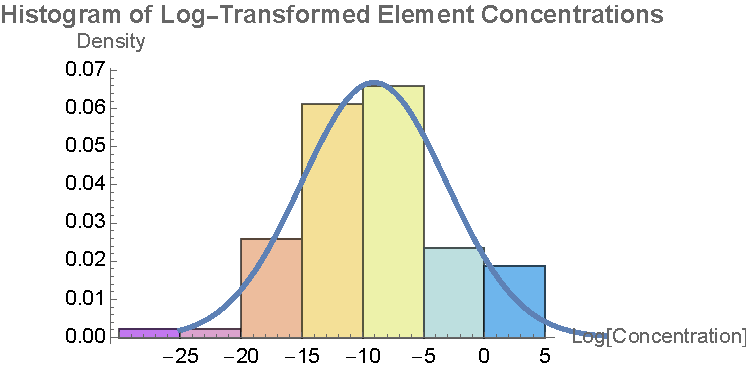
\includegraphics[width=0.7\textwidth]{resources/element_concentration.pdf}
    \caption{地壳中元素浓度的对数分布图}
    \label{fig:lognormal}
\end{figure}\footnote{使用Mathematica绘制,源代码可见
\href{https://github.com/Sazzzzzz/MathNotes/blob/main/code_demos/log_normal_dist_demo.nb}{\texttt{MathNotes/code_demos/log_normal_dist_demo.nb}}}
% TODO: Fix the graph
更多对数正态分布的应用可见
\href{https://en.wikipedia.org/wiki/Log-normal_distribution#Occurrence_and_applications}{Wikipedia}

\subsubsection{\(\chi^{2}\) 分布}
% TODO: Add the definition of Chi-square distribution
\begin{definition}{\(\chi^{2}\) 分布}
    如果独立随机变量\(\xi_{1}, \dots ,\xi_{n}\) 服从标准正态分布\(N(0,1)\),
    则随机变量\(\eta = \xi_{1}^{2} + \xi_{2}^{2} + \cdots +
    \xi_{n}^{2}\) 服从\(\chi^{2}\) 分布,其概率密度函数为:
    \[
        p(x) = \frac{1}{2^{n/2} \gamma{\frac{n}{2}}}
        x^{\frac{n}{2}-1}
        \e^{-\frac{x}{2}}, \quad x>0
        \]
\end{definition}

接下来我们用两种方法推导\(\chi^{2}\) 分布的概率密度函数:
\paragraph{方法一:}
已知标准正态分布的概率密度函数:\[
    p(x) = \frac{1}{\sqrt{2\pi}} \e^{-\frac{x^{2}}{2}}
\]
\begin{align*}
    \P{\eta<y} &= \P{\xi_{1}^{2} + \xi_{2}^{2} + \cdots +
    \xi_{n}^{2} > y} \\
    &= \idotsint\limits_{x_{1}^{2} + x_{2}^{2} + \cdots +
    x_{n}^{2} > y} p(x_{1}) p(x_{2}) \cdots p(x_{n}) \d{x}_{1}
    \d{x}_{2} \cdots \d{x}_{n} \\
    &= \frac{1}{\sqrt{2\pi}^{n}}
    \idotsint\limits_{x_{1}^{2} + x_{2}^{2} + \cdots + x_{n}^{2} > y}
    \e^{-\frac{x_{1}^{2}+ x_{2}^{2} +\dots + x_{n}^{2}}{2}}
    \d{x}_{1} \d{x}_{2} \cdots \d{x}_{n} \\
\end{align*}

作极坐标变换:
% TODO: Fix the position of ellipses
\[
    \begin{cases}
        x_{1} = r \cos \theta_{1} \\
        x_{2} = r \sin \theta_{1} \cos \theta_{2} \\
        \vdots\\
        x_{n-1} = r \sin \theta_{1} \sin \theta_{2} \cdots
        \sin\theta_{n-2} \cos\theta_{n-1}\\
        x_{n} = r \sin\theta_{1} \sin\theta_{2} \cdots
        \sin\theta_{n-2} \sin\theta_{n-1}\\
    \end{cases}
\]
Jacobi行列式为:
\[
    \frac{D(x_{1},\dots ,x_{n})}{D(r,\theta_{1},\dots,
    \theta_{n-1})} = r^{n-1} \sin^{n-2} \theta_{1}
    \sin^{n-3} \theta_{2} \cdots \sin\theta_{n-2}
\]
从而:
\[
    \P{\eta<y} = \frac{2\pi}{\sqrt{2\pi}^{n}}
    \int_{0}^{y} r^{n-1} \e^{-\frac{r^{2}}{2}} \d{r}
    \int_{0}^{\pi} \sin^{n-2} \theta_{1} \d{\theta_{1}} \cdots
    \int_{0}^{\pi} \sin\theta_{n-2} \d{\theta_{n-2}}
\]
其中:
\begin{align*}
    &\placeholder{=}\int_{0}^{\pi} \sin^{n-2} \theta_{1}
    \d{\theta_{1}} \dots
    \int_{0}^{\pi} \sin\theta_{n-2} \d{\theta_{n-2}}\\
    &= \betafunc{\frac{1}{2}}{\frac{n-1}{2}}
    \betafunc{\frac{1}{2}}{\frac{n-2}{2}} \cdots
    \betafunc{\frac{1}{2}}{\frac{1}{2}}\\
    &=
    \frac{\gammafunc{\dfrac{1}{2}}
    \cancel{\gammafunc{\frac{n-1}{2}}}}{\gammafunc{\dfrac{n}{2}}} \cdot
    \frac{\gammafunc{\dfrac{1}{2}}
    \cancel{\gammafunc{\frac{n-2}{2}}}}{\cancel{\gammafunc{\dfrac{n-1}{2}}}}
    \cdots
    \frac{\gammafunc{\dfrac{1}{2}}
    \cancel{\gammafunc{\frac{1}{2}}}}{\cancel{\gammafunc{\dfrac{1}{2}}}}\\
    &= \frac{\sqrt{\pi}^{n-1} }{\gammafunc{\dfrac{n}{2}}}
\end{align*}
于是概率密度函数为:
\begin{align*}
    p(y) &= \frac{2\pi}{\sqrt{2\pi}^{n}} r^{n-1} \e^{-\frac{r^{2}}{2}}
    \cdot \frac{\sqrt{\pi}^{n-1} }{\gammafunc{\dfrac{n}{2}}}\\
    &= \frac{1}{2^{n/2} \gammafunc{\dfrac{n}{2}}}
    y^{\frac{n}{2}-1} \e^{-\frac{y}{2}}, \quad y>0
\end{align*}

实际上,如果注意到积分\(C_{n}=\int_{0}^{\pi} \sin^{n-2} \theta_{1}
    \d{\theta_{1}} \cdots
\int_{0}^{\pi} \sin\theta_{n-2} \d{\theta_{n-2}}\)
只作为系数出现, 则有\[
    F(y)=\P{\eta<y} = C_{n} \int_{0}^{y} r^{n-1}
    \e^{-\frac{r^{2}}{2}} \d{r}
\]
\[
    F(+\infty) = C_{n} \int_{0}^{+\infty} r^{n-1}
    \e^{-\frac{r^{2}}{2}} \d{r} = C_{n} \cdot \sqrt{2}^{n}
    \gammafunc{\frac{n}{2}} = 1
\]
故:
\begin{align*}
    C_{n} &= \frac{1}{\sqrt{2}^{n} \gammafunc{\frac{n}{2}}}\\
    p(y) &= \frac{1}{2^{n/2} \gammafunc{\frac{n}{2}}} y^{\frac{n}{2}-1}
    \e^{-\frac{y}{2}}
\end{align*}

\paragraph{方法二:} 记\(\eta_{i}=\xi_{i}\), 则\(\eta_{i}\)
的分布密度函数为\(q(x)= \frac{1}{\sqrt{2\pi y}}\e^{-\frac{y}{2}}\).
从而\(\L{p(x)}=\frac{1}{\sqrt{2s+1}}\)

\(\eta=\xi_{1}^{2}+ \dots +\xi_{n}^{2} = \eta_{1} +
\dots \eta_{n}\), 记\(\eta\) 的分布密度函数为\(p(x)\),则:
\[
    \L{p(x)} = \L{\underbrace{p(x) * p(x) * \dots *
    p(x)}_{n \text{个}}} =
    \L{p(x)}^{n} = \frac{1}{(2s+1)^{n/2}}
\]
故
\[p(x) = \invL{\frac{1}{(2s+1)^{\frac{n}{2}}}}=
    \frac{1}{2^{n/2} \gammafunc{\dfrac{n}{2}}}
x^{\frac{n}{2}-1} \e^{-\frac{x}{2}}\]

\paragraph{\(\chi^{2}\) 检测与\(\chi^{2}\) 分布的关系}

\href{https://basic.smartedu.cn/tchMaterial/detail?contentType=assets_document&contentId=ffaba6c3-497d-47b0-b91a-784f43625507&catalogType=tchMaterial&subCatalog=tchMaterial}{高中选择性必修三}
时我们就研究过如何列联表判断二元分类变量是否独立。若两变量独立,
我们估计真值与期望差值的绝对值
大小不会很大,并以他们\textbf{标准化后的平方和}作为判断标准。
实际上这就是自由度为\(1\)的\(\chi^{2}\) 分布\UseVerb{smile}

在Mathematica中输入以下代码,立刻就能得到课本上给出的\(5\)个常用的小概率值和相应的临界值!
% https://basic.smartedu.cn/tchMaterial/detail?contentType=assets_document&contentId=ffaba6c3-497d-47b0-b91a-784f43625507&catalogType=tchMaterial&subCatalog=tchMaterial
\begin{lstlisting}[language=Mathematica]
set = {0.1, 0.05, 0.01, 0.005, 0.001}
result =
 Table[Round[InverseCDF[ChiSquareDistribution[1], 1 - x], 0.001], {x,
   set}]
Grid[{Prepend[set, HoldForm[\[Alpha]] // DisplayForm],
  Prepend[result, HoldForm[Subscript[x, \[Alpha]]] // DisplayForm]},
  Frame -> All]
\end{lstlisting}
% TODO: Mimic the table in the book
\begin{table}[H]
    \centering
    \begin{tabular}{|c|c|c|c|c|c|}
        \hline
        \(\alpha\) & 0.1   & 0.05  & 0.01  & 0.005 & 0.001  \\
        \hline
        \(x_{\alpha}\) & 2.706 & 3.841 & 6.635 & 7.879 & 10.828 \\
        \hline
    \end{tabular}
\end{table}

更一般的,对于\(M \times N\) 类型的联表,作\[
    \chi^{2}= \sum_{m=1}^{M} \sum_{n=1}^{N} \frac{(O_{mn} -
    E_{mn})^{2}}{E_{mn}}
\]
那么\(\chi^{2}\) 服从自由度为\((M-1)(N-1)\) 的\(\chi^{2}\) 分布。

\begin{quote}
    可是为什么自由度是\((M-1)(N-1)\) 呢?
\end{quote}

这里给出一个粗浅的解释,自由度的定义参考
\href{https://en.wikipedia.org/wiki/Degrees_of_freedom_(statistics)#Example}{维基百科}。

在\(M \times N\) 的联表中,本身应当有\(MN\) 个自由变量。但是边界分布是已知的,每一列的和,
每一行的和是已知的。但这只会把自由度降低\(M+N-1\)。
因为列边界分布的总和与行边界分布的总和都等于整个表格中所有元素的总和。因此,\(\chi^{2}\)
满足自由度为\(MN-M-N+1 = (M-1)(N-1)\) 的\(\chi^{2}\)分布。

% TODO: Relation between Chi-square and p value
% TODO: F distribution
% TODO: t distribution
% TODO: Cauchy distribution P182 32 是两正态的比
% Laplace分布 Maxwell分布

\subsection{正态分布}
% 正态分布的性质

\subsubsection{正态分布的导出}
% 正态分布在等概率椭圆内的积分
二元正态分布的条件分布、边际分布都是正态分布。
二元正态分布两变量相互独立当且仅当\(\rho=0\)

% TODO: Add deduction of Normal distribution
\subsection{正态分布变量的生成}
\begin{claim}{}
    对于两个相互独立的标准正态分布随机变量\((\xi, \eta)\),
    记\(r=\sqrt{\xi^{2}+\eta^{2}}\), \(\theta =
    \tan^{-1}\left( \frac{\eta}{\xi} \right)\),
    则\(r\)服从\textbf{Rayleigh分布},
    \(\theta\)服从均匀分布\(U(0,2\pi)\)。
\end{claim}

\begin{definition}{Rayleigh分布}
    称\(\xi\) 服从Rayleigh分布,若其概率密度函数为:
    \[
        R(r) = r\e^{-\frac{r^{2}}{2}}, \quad r>0
    \]
\end{definition}

\begin{theorem}{Box-Muller变换}
    设\(U_{1}, U_{2}\) 是独立的标准正态分布随机变量,则:
    \begin{align*}
        \xi &= \sqrt{-2\ln U_{1}} \cos(2\pi U_{2})\\
        \eta &= \sqrt{-2\ln U_{1}} \sin(2\pi U_{2})
    \end{align*}
    则\(\xi, \eta\) 相互独立且服从标准正态分布。
\end{theorem}

\begin{proof}
    记\(V=\sqrt{-2 \ln U_{1}}\),有\(U_{1}=
    \e^{-\frac{V^{2}}{2}}\),则\(V\) 的概率密度函数为:
    \[
        p(v) = \abs{\left(\e^{-\frac{x^{2}}{2}} \right)'} =
        \e^{-\frac{v^{2}}{2}} v, \quad v>0
    \]
    故\(V\) 服从Rayleigh分布。从而\(\xi,\eta\) 服从标准正态分布。
\end{proof}
\begin{figure}[H]
    \centering
    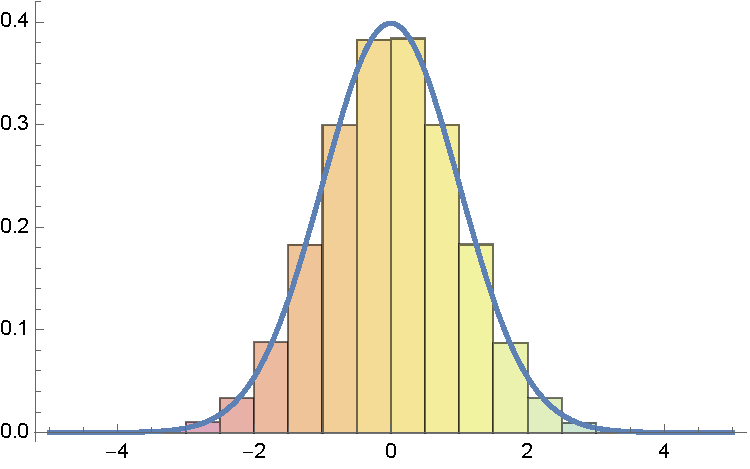
\includegraphics[width=0.7\textwidth]{resources/box_muller_transform.pdf}
    \caption{Box-Muller变换生成的随机变量与标准正态分布}
\end{figure}

\subsection{二元正态分布在椭圆内的积分}

\subsubsection{等概率椭圆内的积分}

\begin{problem}{二元正态分布在等概率椭圆内的积分}
    若\((\xi,\eta)\) 服从二元正态分布,参数为\(\mu_{1}\),\(\mu_{2}\),
    \(\sigma_{1}^{2}\),\(\sigma_{2}^{2}\),\(\rho\),
    记椭圆\(D(\lambda)\):\[
        \frac{(x-\mu_{1})^{2}}{\sigma_{1}^{2}} +
        \frac{(y-\mu_{2})^{2}}{\sigma_{2}^{2}} \leq \lambda^{2}
    \]
    求\(\P{(\xi,\eta) \in D(\lambda)}\)。
\end{problem}

\begin{proof}
    记:
    \begin{equation}
        \begin{cases}
            u = \frac{x}{\sigma_{1}} - \frac{\rho y}{\sigma_{2}}\\
            v = \frac{y\sqrt{1-\rho^{2}}}{\sigma_{2}}
        \end{cases}
    \end{equation}
    则:
    \begin{align*}
        \P{(\xi,\eta) \in D(\lambda)} &=
        \iint\limits_{(x,y) \in D(\lambda)}
        p(x,y) \d{x} \d{y}\\
        &= \frac{1}{2\pi(1-\rho^{2})} \iint\limits_{u^{2} +
        v^{2} \leq \lambda^{2}}
        \e^{-\frac{1}{2(1-\rho^{2})}\left(u^{2} +
        v^{2}\right)} \d{u} \d{v}\\
        &= \frac{1}{2\pi(1-\rho^{2})} \int_{0}^{2\pi} \d{\theta}
        \int_{0}^{\lambda} \e^{-\frac{r^{2}}{2(1-\rho^{2})}} r \d{r}\\
        &= 1- \e^{-\frac{\lambda^{2}}{2(1-\rho^{2})}}
    \end{align*}
\end{proof}

这可以看作是一种瑞利分布的推广。

\paragraph{一般情况下的积分}
不失一般性,考虑二元标准正态分布在椭圆\(\frac{x^{2}}{a^{2}} +
\frac{y^{2}}{b^{2}} =\lambda^{2}\) 内的积分:
\begin{align*}
    &\placeholder{=} \int\limits_{\frac{x^{2}}{a^{2}} +
        \frac{y^{2}}{b^{2}} \leq
    \lambda^{2}} \frac{1}{2\pi} \e^{-\frac{1}{2}\left(
    x^{2}+y^{2} \right)}  \d{x} \d{y}\\
    &= \frac{1}{2\pi} \int_{0}^{2\pi} \d{\theta}
    \int_{0}^{\frac{a^{2}b^{2}}{b^{2}\cos^{2}\theta
    \sin^{2}\theta}} \e^{-\frac{r^{2}}{2}} r\d{r} \\
    &= 1- \frac{2}{\pi} \int_{0}^{\frac{\pi}{2}}
    \e^{-\frac{1}{2} \cdot
    \frac{b^{2}}{1-e^{2}\cos^{2}\theta}} \d{\theta}\\
    & \cdots \cdots
\end{align*}
\footnote{另一种思路是考虑二元正态分布的分布函数为\(F(x,y) = \frac{1}{4}
        \left(1- \erf(-\frac{x}{\sqrt{2}}) \right)\left( 1-
\erf(-\frac{y}{\sqrt{2}}) \right) \),利用积分与边界的性质计算}

\texttt{其实我也还没算出来\UseVerb{naughty}}
